
\section{Introduction}

	Many top cathode \gls{ito}\-/\gls{pedotpss}\-/\gls{mapi}\-/\gls{pcbm70}\-/\ch{Ag} perovskite solar cells have been fabricated.
	The thickness of each of \gls{pedotpss} (\gls{htm}), \gls{mapi} (absorber), and \gls{pcbm70} (\gls{etm}) has been independently varied.
	All these layers were deposited by spin coating and the thickness was tuned \textsl{via} spin coating speed.
	These parameters where chosen so that their variation affect as little as possible the rest of the solar cell stack, so that we can unequivocally relate the observations to the changes.
	The champion device performances of each configuration are listed in \cref{table:thicknesses_jv}.


	\paragraph{Design of the Experiment}
	Perovskite synthesis is a very easy and fragile process at the same time.
	When varying a fabrication parameter, for example during an optimization, it is quite likely to provoke a "butterfly effect" with the resulting device differing from the reference by much more than the characteristic under study.
	A principal component analysis of the fabrication parameters would be needed for a rational optimization, but such a complex procedure is further hindered by the difficulty of identifying all relevant contributions.
	In this study we vary a set of parameters that hopefully have a foreseeable relation with the resulting device structure: thickness of each layer, through the tuning of the spin coating deposition speed.
	This variation should just affect the thickness of one layer, having just a minor influence on the other layers and the rest of the device physical features.
	This will allow us to univocally relate the observations to the modifications.

	\paragraph{Author contributions}
	The devices were fabricated and characterised by me under the supervision of Dr.\ Nuria F.\ Montcada, Dr.\ Lydia Cabau, and Prof.\ Emilio J.\ Palomares Gil (fabrication described in \cpagerefrange{methods_top}{methods_top_end}).
	The data was analysed by me and Dr.\ Nuria F.\ Montcada.
	The experiment was designed and the data interpreted by me, Dr.\ Nuria F.\ Montcada, and Prof.\ Emilio J.\ Palomares Gil.



\section{Varying \glsentrytext{mapi} Thickness (Absorber Layer)}

	\begin{figure}
		\makebox[\textwidth][c]{
			\parbox{1.1\textwidth}{
				\centering
				\begin{subfigure}[t]{0.51\textwidth}
					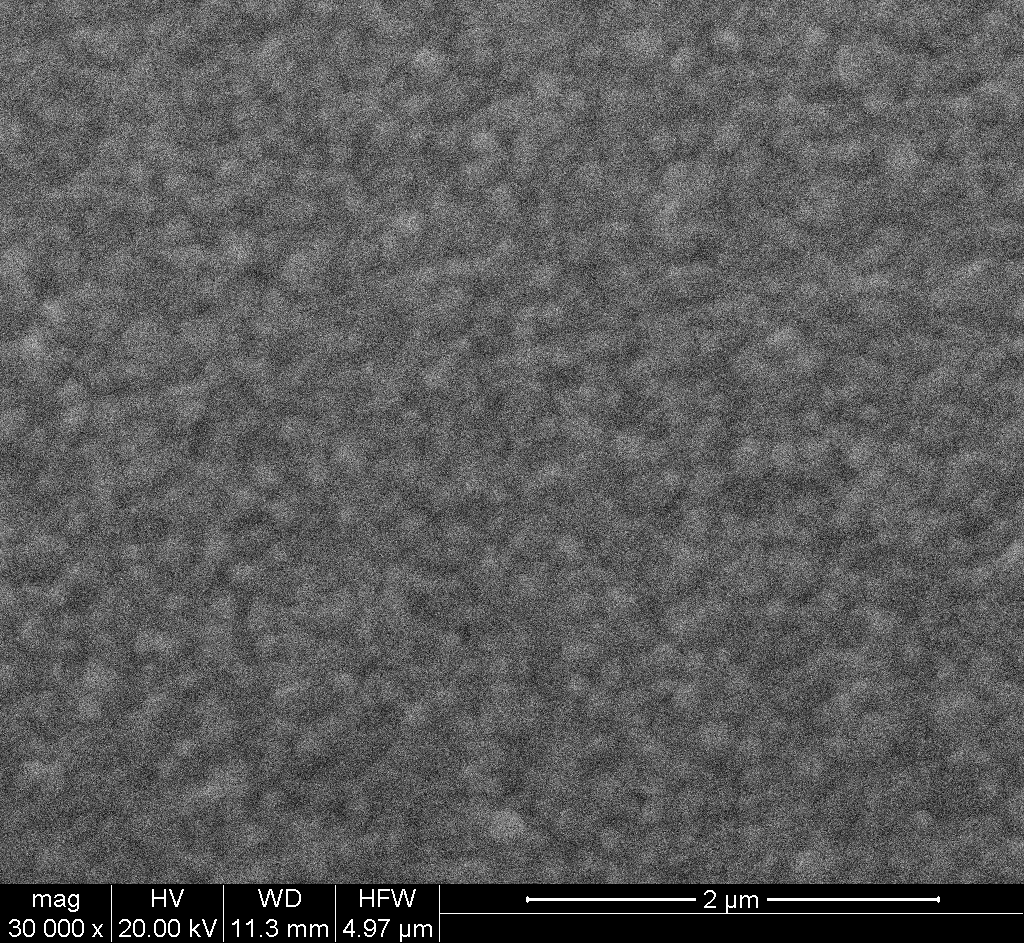
\includegraphics[width=1\textwidth]{esem-topview/ig87-c39-8000RPM-30k-hv-contrast.png}
					\subcaption{\SI{8000}{\rpm}, \SI{230}{\nm}}\label{fig:thicknesses-esem-topview-8000RPM}
				\end{subfigure}
				\qquad
				\begin{subfigure}[t]{0.51\textwidth}
					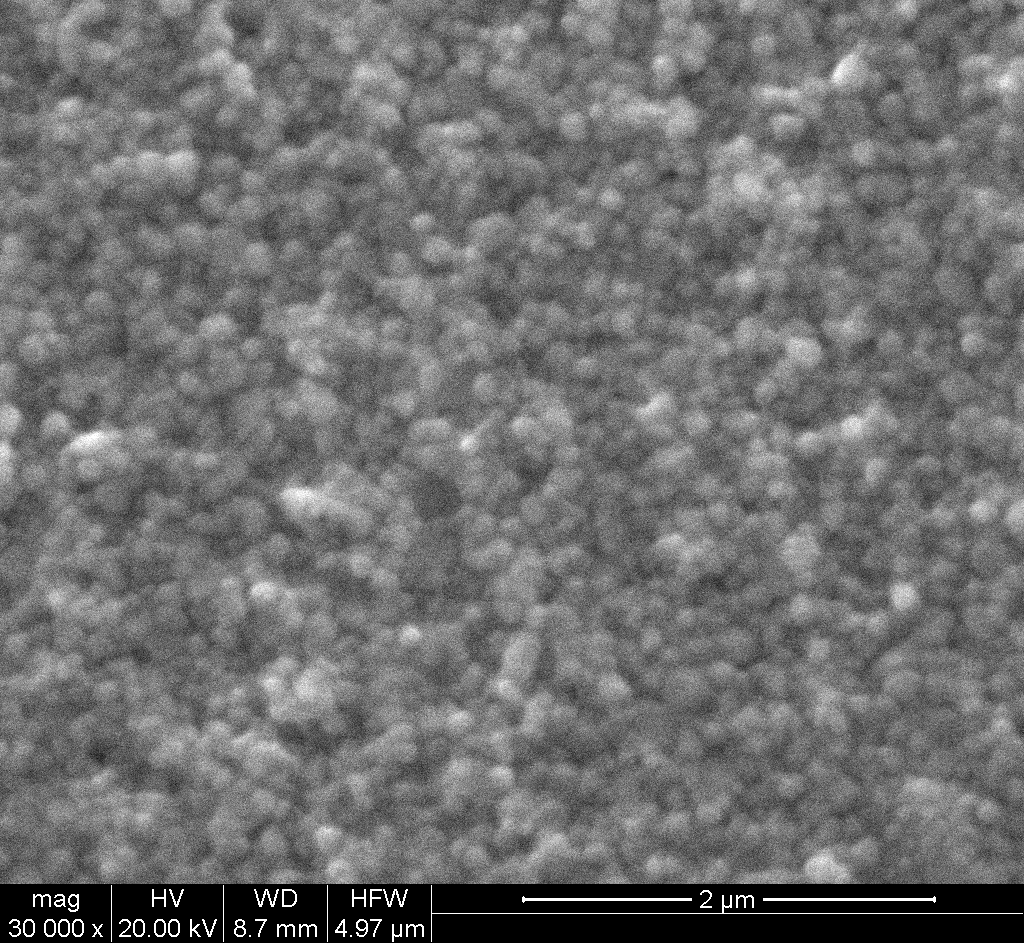
\includegraphics[width=1\textwidth]{esem-topview/ig87-b78-4100RPM-30k-hv-contrast.png}
					\subcaption{\SI{4100}{\rpm}, \SI{320}{\nm}}\label{fig:thicknesses-esem-topview-4100RPM}
				\end{subfigure}
				\bigskip

				\begin{subfigure}[t]{0.51\textwidth}
					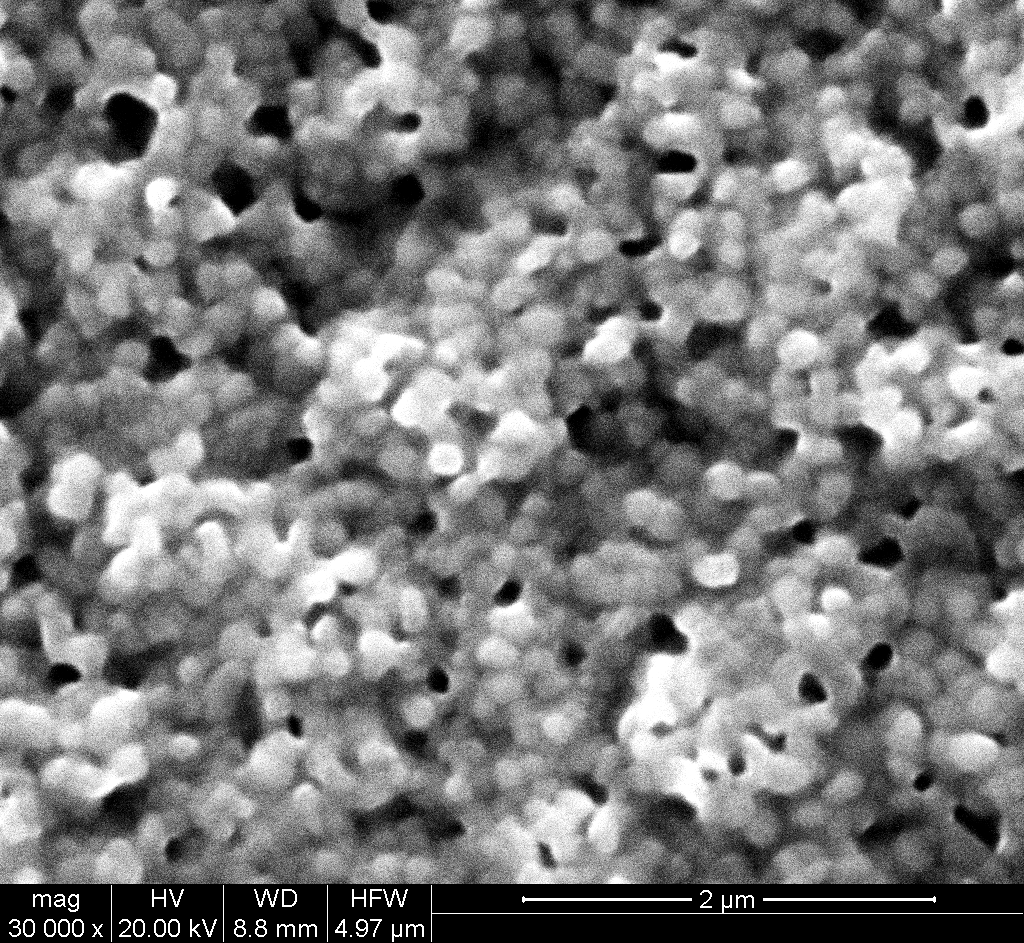
\includegraphics[width=1\textwidth]{esem-topview/ig87-c34-2000RPM-30k-hv-contrast.png}
					\subcaption{\SI{2000}{\rpm}, \SI{440}{\nm}}\label{fig:thicknesses-esem-topview-2000RPM}
				\end{subfigure}
				\mycaption[Top view ESEM images of annealed perovskite layers with various thicknesses.]{
					The surface of a thin perovskite layer is studied using  FIJI/ImageJ \cite{Schindelin2012} on images of two different devices for each deposition condition (just one reported here for brevity).
					The average domain diameter (and its standard deviation) is \SI{182 \pm 25}{\nm} for the thin \SI{230}{\nm} perovskite layer in (\textbf{a}), \SI{190 \pm 34}{\nm} for the medium \SI{320}{\nm} perovskite layer in (\textbf{b}), \SI{189 \pm 23}{\nm} for the thick \SI{440}{\nm} perovskite layer in (\textbf{c}).
				}\label{fig:thicknesses-esem-topview}
			}
		}
	\end{figure}

	\paragraph{Roughness and grain size}
	Using different spin coating speeds, devices with various \gls{mapi} thicknesses were obtained, as detailed in \cref{table:mapi_thickness}.
	As a consequence to the different deposition conditions, the \gls{mapi} surface is more rough for the thick device than for the thin one, as can be intuited looking at \gls{esem} image in \cref{fig:thicknesses-esem-topview}.
	Any way, measuring the roughness average with a profilometer, it resulted to be \SI{< 10}{\nm} for all the cases, so the \SI{40}{\nm} \gls{pcbm70} layer should be enough for an homogeneous coverage.
	From the same \gls{esem} image, we can measure the grain lateral size, which is not significantly different for the six observed samples (two per each \gls{mapi} thickness, data detailed in \cref{fig:thicknesses-esem-topview} caption).

	%\begin{table}%[h]	% longtables cannot stay inside a float, otherwise they will not break
	\begin{xltabular}[c]{1.05\linewidth}{@{}>{\hsize=1.2\hsize}Y|>{\hsize=0.9\hsize}Y|>{\hsize=0.9\hsize}Y | c >{\hsize=1.5\hsize}Y >{\hsize=0.95\hsize}Y >{\hsize=0.75\hsize}Y >{\hsize=0.8\hsize}Y @{}}
		% multirow does not get the correct number of rows with tabularx
		% mycaption does not work inside xltabular
		\caption[Layers thicknesses and related average performances of top cathode cells.]{\textbf{Layers thicknesses and related average performances of top cathode cells.}
			Explored thicknesses with \textit{average} forward and reverse J-V sweep performances.
			The standard deviation for each value is indicated after the $\pm$ symbol.
			For each reported result, at least 8, 8, and 4 devices were averaged respectively for \gls{mapi}, \gls{pcbm70}, and \gls{pedotpss} thickness exploration.
			\Gls{etm} column indicates the \gls{pcbm70} thickness, while \acr{htm} one refers to \gls{pedotpss} thickness.
			The measurement conditions were \SI{1}{sun} illumination, no light soaking, \SI{1}{\V\per\s} sweep speed.
			A boxplot representation of this data can be found in \authoryear{Gelmetti2017}.
			J-V curve for record devices are reported in \cref{fig:thicknesses-jv_champions-mapi,fig:thicknesses-jv_champions-pcbm,fig:thicknesses-jv_champions-pedotpss}.
		}\label{table:thicknesses_jv}\\[\belowcaptionskip]
		\multicolumn3{c|}{\small\textbf{Layers thickness}} & \multicolumn{5}{c}{\small\textbf{J-V sweep parameters}}
		\rule[-1ex]{0pt}{3ex} \\
		\small\gls{mapi} &  \small\gls{etm} & \small\gls{htm} &\small Sweep & \small\gls{jsc} &  \small\gls{voc} & \small\gls{ff} &  \small\gls{pce} \\
		\rule[-1ex]{0pt}{2.5ex}  \footnotesize\si{\nm} &  \footnotesize\si{\nm} &  \footnotesize\si{\nm} & - & \footnotesize\si{\mA\per\square\cm} &  \footnotesize\si{\V} & \footnotesize\si{\%} &  \footnotesize\si{\%} \\[1mm]
		\hline
		\endfirsthead
		\multicolumn{2}{@{}l}{\ldots \small continues}\\
		\hline
		\small\gls{mapi} & \small\gls{etm} & \small\gls{htm} &\small Sweep & \small\gls{jsc} & \small\gls{voc} & \small\gls{ff} & \small\gls{pce} \\
		\hline
		\endhead
		\hline
		\multicolumn{8}{r@{}}{\small continues\ldots}\\
		\endfoot
		\hline
		\endlastfoot
		\rule[-1ex]{0pt}{3ex}
		\multirow{3}{*}{230} 	& \multirow{11}{*}{40}	&  \multirow{11}{*}{65}	&fwd	&	13.5	$\pm	0.5	$ & 	1.03	$\pm	0.01	$ & 	53	$\pm	3	$ & 	7.3	$\pm	0.4	$ \\*
		\rule[-1ex]{0pt}{2.5ex}
		&  						& 						&rev	&	13.6	$\pm	0.5	$ & 	1.02	$\pm	0.01	$ & 	55	$\pm	3	$ & 	7.7	$\pm	0.5	$ \\*
		\cline{1-1} \cline{4-8}
		\multirow{3}{*}{320}	&  						&  						&fwd	&	13.9	$\pm	0.3	$ & 	1.04	$\pm	0.01	$ & 	57	$\pm	5	$ & 	8.2	$\pm	0.6	$ \\*
		\rule[-1ex]{0pt}{2.5ex}
		&  						&  						&rev	&	14.1	$\pm	0.3	$ & 	1.04	$\pm	0.01	$ & 	55	$\pm	4	$ & 	8.1	$\pm	0.5	$ \\*
		\cline{1-1} \cline{4-8}
		\multirow{3}{*}{440}	&  						&  						&fwd	&	16.3	$\pm	2.1	$ & 	1.01	$\pm	0.04	$ & 	58	$\pm	2	$ & 	9.5	$\pm	0.8	$ \\*
		\rule[-1ex]{0pt}{2.5ex}
		&  						&  						&rev	&	16.5	$\pm	1.9	$ & 	0.98	$\pm	0.07	$ & 	50	$\pm	5	$ & 	8.1	$\pm	1.4	$ \\[1mm]
		\hline
		\multirow{15}{*}{350}	& \multirow{3}{*}{40} 	&  \multirow{15}{*}{65} &fwd	&	16.4	$\pm	2.2	$ & 	0.93	$\pm	0.06	$ & 	48	$\pm	8	$ & 	7.4	$\pm	1.8	$ \\*
		&  						&  						&rev	&	16.1	$\pm	2.1	$ & 	0.95	$\pm	0.06	$ & 	50	$\pm	5	$ & 	7.6	$\pm	1.4	$ \\*
		\cline{2-2} \cline{4-8}
		& \multirow{3}{*}{60} 	& 					 	&fwd	&	13.2	$\pm	1.1	$ & 	0.99	$\pm	0.04	$ & 	47	$\pm	6	$ & 	6.2	$\pm	1.1	$ \\*
		&  						&  						&rev	&	12.8	$\pm	0.7	$ & 	0.98	$\pm	0.05	$ & 	47	$\pm	5	$ & 	5.9	$\pm	0.8	$ \\*
		\cline{2-2} \cline{4-8}
		& \multirow{3}{*}{90} 	&  						&fwd	&	11.1	$\pm	0.6	$ & 	1.03	$\pm	0.03	$ & 	42	$\pm	2	$ & 	4.8	$\pm	0.6	$ \\*
		&  						&  						&rev	&	11.1	$\pm	0.8	$ & 	1.00	$\pm	0.04	$ & 	44	$\pm	2	$ & 	4.8	$\pm	0.5	$ \\*
		\cline{2-2} \cline{4-8}
		& \multirow{3}{*}{120} 	&  						&fwd	&	7.7	$\pm	1.6	$ & 	1.02	$\pm	0.04	$ & 	18	$\pm	2	$ & 	1.4	$\pm	0.4	$ \\*
		&  						&  						&rev	&	7.6	$\pm	1.6	$ & 	1.01	$\pm	0.04	$ & 	18	$\pm	2	$ & 	1.4	$\pm	0.4	$ \\[1mm]
		\hline
		\multirow{11}{*}{300}	& \multirow{11}{*}{40}	& \multirow{3}{*}{27} 	&fwd	&	12.3	$\pm	1.5	$ & 	1.04	$\pm	0.03	$ & 	55	$\pm	9	$ & 	6.9	$\pm	0.8	$ \\*
		&  						&  						&rev	&	11.9	$\pm	1.7	$ & 	1.03	$\pm	0.04	$ & 	54	$\pm	11	$ & 	6.6	$\pm	0.7	$ \\*
		\cline{3-8}
		&  						& \multirow{3}{*}{45} 	&fwd	&	12.2	$\pm	1.7	$ & 	1.04	$\pm	0.01	$ & 	58	$\pm	4	$ & 	7.3	$\pm	1.2	$ \\*
		&  						&  						&rev	&	11.8	$\pm	1.7	$ & 	1.00	$\pm	0.09	$ & 	53	$\pm	7	$ & 	6.2	$\pm	0.9	$ \\*
		\cline{3-8}
		& 				 		& \multirow{3}{*}{65} 	&fwd	&	12.4	$\pm	1.6	$ & 	1.04	$\pm	0.02	$ & 	60	$\pm	3	$ & 	7.7	$\pm	0.6	$ \\*
		&  						&  						&rev	&	12.6	$\pm	1.4	$ & 	1.00	$\pm	0.10	$ & 	60	$\pm	4	$ & 	7.5	$\pm	0.4	$ \\[1mm]
	\end{xltabular}

	\paragraph{Current-voltage sweeps}
	In \cref{fig:thicknesses-jv_champions-mapi} we can observe the current-voltage sweeps of the champion devices while in \cref{table:thicknesses_jv} the averages and standard deviations are reported.
	The \gls{ff} is not significantly different for the devices with different \gls{mapi} layer thickness.
	The only observable difference is the presence of a higher hysteresis\index{hysteresis} (difference between forward and reverse scan) in this parameter for the thicker \gls{mapi} case.
	This could indicate a small change in the perovskite\-/\gls{pcbm70} interface or just a change in the hysteresis\index{hysteresis} characteristic time due to the increased ionic resistance in the thicker \gls{mapi} layer.
	Regarding the \gls{voc}, this value also did not change with thickness, indicating that the same recombination processes and dynamics are present disregarding the absorber thickness.
	The higher deviation of this parameter for the thicker perovskite could be due to its higher roughness, causing some devices to have pinholes in the \acr{etm} layer.
	What is clear and expected is the \gls{jsc} increase.
	This is most likely due to the low \gls{eqe} in the thin perovskite layer due to its far\hyp{}from\hyp{}zero transmittance.
	The increase in photogeneration rate is reflected in an increase of \gls{pce}.

	\begin{SCfigure}
		\centering
		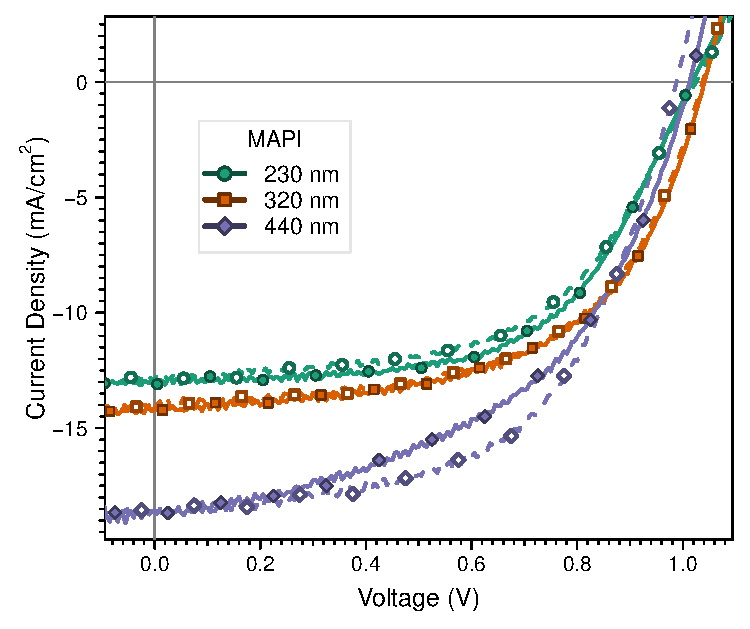
\includegraphics[width=0.8\textwidth]{jv_champions-mapi/mapi-IVs.pdf}
		\mycaption[Current-voltage sweeps for champion devices with different MAPI thicknesses.]{The solid line with filled markers represents the forward scan, while the dashed line with hollow markers represents the reverse scan.}\label{fig:thicknesses-jv_champions-mapi}
	\end{SCfigure}


	%\afterpage{
	\begin{table}%[h]	% longtables cannot stay inside a float, if they do, they will not break
		\caption[Parameters fitted from CE and DC data, from devices with different layers' thicknesses.]{\textbf{Parameters fitted from CE and DC data, from devices with different layers' thicknesses.}
			The experimental data reported in \cref{fig:thicknesses-mapi-geometric,fig:thicknesses-pcbm-geometric,fig:thicknesses-pedotpss-geometric} has been fitted using \cref{eq:ce_full} for \acr{ce} data and \cref{eq:dc_full} for \acr{dc} data.
		}\label{table:thicknesses_photophysics}
		\centering
		\begin{tabularx}{1.05\linewidth}{@{} >{\hsize=1.1\hsize}Y | >{\hsize=0.7\hsize}Y | >{\hsize=0.7\hsize}Y | Y >{\hsize=1.65\hsize}Y >{\hsize=0.6\hsize}Y | Y  >{\hsize=1.65\hsize}Y >{\hsize=0.6\hsize}Y @{}}
			% multirow does not get the correct number of rows with tabularx
			% mycaption does not work inside xltabular
			%		\\[\belowcaptionskip]
			\multicolumn3{c|}{\small\textbf{Layers thickness}} & \multicolumn{3}{c|}{\small\textbf{CE}} & \multicolumn{3}{c}{\small\textbf{DC}}
			\rule[-1ex]{0pt}{3ex}                                                                                                                                                                                                                                                                                                                                              \\
			\small\gls{mapi}                                   & \small\gls{etm}                        & \small\gls{htm}                       & \small\gls{symb:Cg}                     & \small\gls{symb:neq}                     & \small\gls{symb:m}       & \small\gls{symb:Cg}                     & \small\gls{symb:neq}                     & \small\gls{symb:m}      \\
			\rule[-1ex]{0pt}{2.5ex}  \footnotesize\si{\nm}     & \footnotesize\si{\nm}                  & \footnotesize\si{\nm}                 & \footnotesize\si{\nano\F\per\square\cm} & \footnotesize\si{\coulomb\per\square\cm} & -                        & \footnotesize\si{\nano\F\per\square\cm} & \footnotesize\si{\coulomb\per\square\cm} & -                       \\[1mm]
			\hline
			\rule[-1ex]{0pt}{4ex}
			230                                                & \multirow{3}{*}{40}                    & \multirow{3}{*}{65}                   & \rnum{85.3301567640111}                 & \rnum{5.12603766463996e-21}              & \rnum{1.42540882502849}  & \rnum{63.5691599645725}                 & \rnum{2.80156436794216e-12}              & \rnum{4.42885311532801} \\*
			\cline{1-1} \cline{4-9}
			\rule[-1ex]{0pt}{4ex}
			320                                                &                                        &                                       & \rnum{77.7280226931573}                 & \rnum{4.82359451755698e-27}              & \rnum{0.970504332684817} & \rnum{55.4099677743798}                 & \rnum{9.01531708758845e-13}              & \rnum{4.09817044704697} \\*
			\cline{1-1} \cline{4-9}
			\rule[-1ex]{0pt}{4ex}
			440                                                &                                        &                                       & \rnum{70.7196355753457}                 & \rnum{1.1916876016195e-27}               & \rnum{0.912575007143644} & \rnum{50.42918432699}                   & \rnum{8.6536760550073e-15}               & \rnum{2.64532408455481} \\
			\hline
			\rule[-1ex]{0pt}{4ex}
			\multirow{3}{*}{350}                               & 40                                     & \multirow{3}{*}{65}                   & \rnum{76.399963266735}                  & \rnum{2.59099124009742e-20}              & \rnum{1.42377526492346}  & \rnum{55.0987488891515}                 & \rnum{7.87748762963633e-15}              & \rnum{2.51025076329765} \\*
			\cline{2-2} \cline{4-9}
			\rule[-1ex]{0pt}{4ex}
			                                                   & 60                                     &                                       & \rnum{61.3214241914314}                 & \rnum{9.01470965786247e-25}              & \rnum{1.07005213324604}  & \rnum{42.8290117954868}                 & \rnum{9.34331162626908e-13}              & \rnum{3.81783541577789} \\*
			\cline{2-2} \cline{4-9}
			\rule[-1ex]{0pt}{4ex}
			                                                   & 90                                     &                                       & \rnum{43.8300398524054}                 & \rnum{5.33438024104082e-29}              & \rnum{0.853781763130922} & \rnum{33.9400710508692}                 & \rnum{4.49280198629451e-11}              & \rnum{5.98365652726317} \\
			\hline
			\rule[-1ex]{0pt}{4ex}
			\multirow{3}{*}{300}                               & \multirow{3}{*}{40}                    & 27                                    & \rnum{63.8554990179897}                 & \rnum{9.74708581977915e-15}              & \rnum{2.93729998552211}  & \rnum{46.1396721657447}                 & \rnum{1.63620664547478e-15}              & \rnum{2.37232492243424} \\*
			\cline{3-9}
			\rule[-1ex]{0pt}{4ex}
			                                                   &                                        & 45                                    & \rnum{66.7217372609922}                 & \rnum{6.39620737296978e-21}              & \rnum{1.2951381459487}   & \rnum{49.8531675841145}                 & \rnum{4.64793103413763e-16}              & \rnum{2.13846267623868} \\*
			\cline{3-9}
			\rule[-1ex]{0pt}{4ex}
			                                                   &                                        & 65                                    & \rnum{64.4501923191207}                 & \rnum{5.44744643856892e-32}              & \rnum{0.678974589798595} & \rnum{50.3194494652546}                 & \rnum{1.34432980262899e-16}              & \rnum{2.00044590997543} \\
		\end{tabularx}
	\end{table}
	%}

	\paragraph{Geometric capacitance from DC and CE}
	From the low and mid background light capacitance obtained from \acr{dc} in \cref{fig:thicknesses-mapi-geometric-dc} and from the linear part of \acr{ce} in \cref{fig:thicknesses-mapi-geometric-ce} we can obtain a geometric capacitance\index{geometric capacitance} $C_|g|$, as explained in \cref{ch:characterization}.
	This capacitance arises from the accumulation of charges in the selective contacts' depletion\index{space charge layer} layers, considering this as a parallel plates capacitor it is easy to foresee that the increase of \gls{mapi} layer will increase the distance between the "plates" and cause a decrease in the capacitance.
	Please note that this is valid just if the \acr{ce} is integrated over short times, so that the ionic displacement is negligible.
	Otherwise, as explained in \cpageref{ce_ions_linear}, the measured geometric capacitance\index{geometric capacitance} would regard charges (ionic and electronic) accumulating on the two sides of each perovskite\-/contact interface (a junction capacitance rather than a geometric capacitance\index{geometric capacitance}), being insensitive to the \gls{mapi} thickness.
	The fitted values of $C_|g|$ are reported in \cref{table:thicknesses_photophysics}.


	\begin{figure}
		\makebox[\textwidth][c]{
			\parbox{1.1\textwidth}{
				\centering
				\begin{subfigure}[t]{0.51\textwidth}
					\includegraphics[width=1.05\textwidth]{photophysics-mapi/photophysics-CEs.pdf}
					\subcaption{Charge from \acr{ce}}\label{fig:thicknesses-mapi-geometric-ce}
				\end{subfigure}
				\qquad
				\begin{subfigure}[t]{0.51\textwidth}
					\includegraphics[width=1.05\textwidth]{photophysics-mapi/photophysics-DCs-capacitance.pdf}
					\subcaption{Capacitance from \acr{dc}}\label{fig:thicknesses-mapi-geometric-dc}
				\end{subfigure}
				\mycaption[CE and DC of devices with different MAPI thicknesses, highlighting the varying geometric capacitance\index{geometric capacitance}.]{
					In (\textbf{a}) the charge \textsl{versus} light bias as obtained from \acr{ce} is reported. The upper solid lines are exponential fittings following \cref{eq:ce_full} while the bottom solid lines show just the exponential part, ignoring the geometric capacitance\index{geometric capacitance}. In (\textbf{b}) the capacitance dependence on light bias is reported as obtained from \acr{dc}. The solid line indicates the fitting using \cref{eq:dc_full}. All the fitted parameters are reported in \cref{table:thicknesses_photophysics}.
				}\label{fig:thicknesses-mapi-geometric}
			}
		}
	\end{figure}


\section{Varying \glsentrytext{pcbm70} Thickness (\glsentryshort{etm} Layer)}
	Using different spin coating speeds, devices with various \gls{pcbm70} thicknesses were obtained, as detailed in \cref{table:pcbm_thickness}.
	This was deposited on top of a rather thin layer of \SI{350}{\nm} of \gls{mapi}, which resulted to be smooth enough to allow the \gls{pcbm70} to homogeneously cover it.

	\begin{SCfigure}
		\centering
		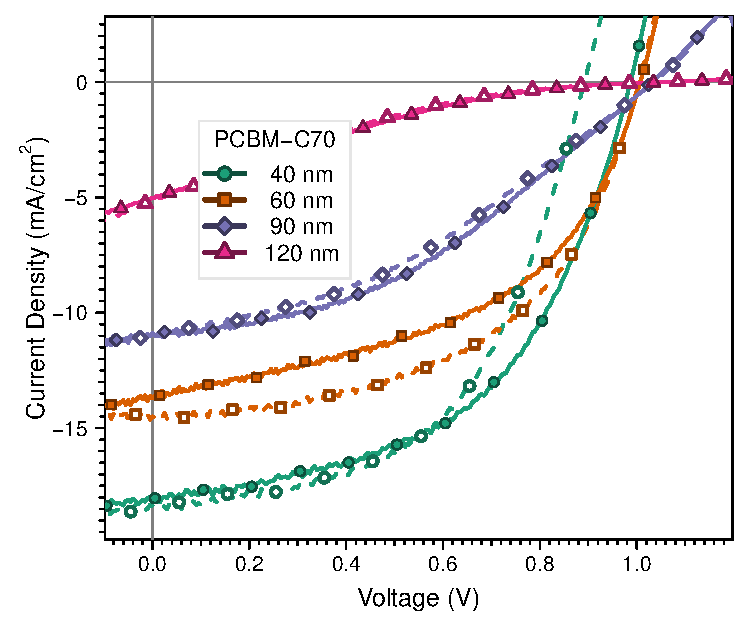
\includegraphics[width=0.8\textwidth]{jv_champions-pcbm/pcbm-IVs.pdf}
		\mycaption[Current-voltage sweeps for champion devices with different \glsentrytext{pcbm70} thicknesses.]{The solid line with filled markers represents the forward scan, while the dashed line with hollow markers represents the reverse scan.}\label{fig:thicknesses-jv_champions-pcbm}
	\end{SCfigure}

	\paragraph{Current-voltage sweeps}
	In \cref{fig:thicknesses-jv_champions-pcbm} we can observe the current-voltage sweeps of the champion devices while in \cref{table:thicknesses_jv} the averages and standard deviations are reported.
	The \gls{ff} is heavily affected by the high series resistance of the thicker \gls{pcbm70} layer.
	The S-shape observed close to \gls{voc} in the current\hyp{}voltage sweep of devices with thick \acr{etm} layer is due to the poor mobility of electrons in \gls{pcbm70} \cite{VonHauff2005} which causes a charges collection bottleneck \cite{Wheeler2015}.
	Interestingly enough, the \gls{voc} slightly increases when the \gls{pcbm70} thickness is increased.
	If confirmed with a stronger statistics, the lower voltage for the thinner layer case could be explained by the presence of some uncovered perovskite area, causing a leakage current between the perovskite and the silver metal electrode.
	As also observed by \authoryear{Seo2014}, increasing the \gls{pcbm70} layer results in a strong decrease of the \gls{jsc}.
	In \authoryear{Shao2016}, the same dependency is observed in disordered \gls{pcbm70} films while it is not present if the layer is solvent annealed.
	Indeed, a very large series resistance, caused by the thick \acr{etm} layer, is expected to affect the short circuit current (this can be seen substituting $V=0$ in the implicit function in \cref{eq:series_resistance}).
	This influence, together with the higher \gls{ff} results in a much higher \gls{pce} for devices with a thin \gls{etm}.

	\begin{figure}
		\makebox[\textwidth][c]{
			\parbox{1.1\textwidth}{
				\centering
				\begin{subfigure}[t]{0.51\textwidth}
					\includegraphics[width=1.05\textwidth]{photophysics-pcbm/photophysics-CEs.pdf}
					\subcaption{Charge from \acr{ce}}\label{fig:thicknesses-pcbm-geometric-ce}
				\end{subfigure}
				\qquad
				\begin{subfigure}[t]{0.51\textwidth}
					\includegraphics[width=1.05\textwidth]{photophysics-pcbm/photophysics-DCs-capacitance.pdf}
					\subcaption{Capacitance from \acr{dc}}\label{fig:thicknesses-pcbm-geometric-dc}
				\end{subfigure}
				\mycaption[CE and DC of devices with different \glsentrytext{pcbm70} thicknesses, highlighting the varying geometric capacitance\index{geometric capacitance}.]{
					In (\textbf{a}) the charge \textsl{versus} light bias as obtained from \acr{ce} is reported.
					The upper solid lines are exponential fittings following \cref{eq:ce_full} while the bottom solid lines show just the exponential part, ignoring the geometric capacitance\index{geometric capacitance}.
					In (\textbf{b}) the capacitance dependence on light bias is reported as obtained from \acr{dc}.
					The solid line indicates the fitting using \cref{eq:dc_full}. All the fitted parameters are reported in \cref{table:thicknesses_photophysics}.
				}\label{fig:thicknesses-pcbm-geometric}
			}
		}
	\end{figure}

	\paragraph{Geometric capacitance from \glsentryshort{dc} and \glsentryshort{ce}}
	Also in the case of increasing \gls{pcbm70} \acr{etm} thickness, the geometric capacitance\index{geometric capacitance} diminishes (observed \textsl{via} \acr{ce} in \cref{fig:thicknesses-pcbm-geometric-ce} and \acr{dc} in \cref{fig:thicknesses-pcbm-geometric-dc}), coherently to what observed by \authoryear{Wheeler2017}.
	Thinking within the parallel plate capacitor model (explained in \cpageref{geometric_capacitance}) where $C_|g| = \epsilon_0 \epsilon_|r| A / d$, this means that the distance $d$ between the two charge storage locations is increasing.
	This is incompatible with what we expected: that the electronic charge gets stored in a thin depletion\index{space charge layer} layer in the \acr{etm} on the perovskite layer side, as in this case the distance $d$ would not change increasing the \gls{pcbm70} layer.
	So, the main electrons storage location is either close to the \gls{etm}\-/\ch{Ag} interface or within the whole \acr{etm} layer due to a Debye length (a.k.a. Thomas–Fermi screening length, is an indication of the depth inside a semiconductor layer at which an external electric field is completely screened, it depends on the permittivity and the doping density of the material, see \cpageref{intro-space_charge}) larger than the \gls{pcbm70} thickness.
	So we can consider the \gls{mapi}\-/\gls{pcbm70} stack as the inter\hyp{}electrodes material of a capacitor.


\section{Varying \glsentrytext{pedotpss} Thickness (\glsentryshort{htm} Layer)}

	\begin{SCfigure}
		\centering
		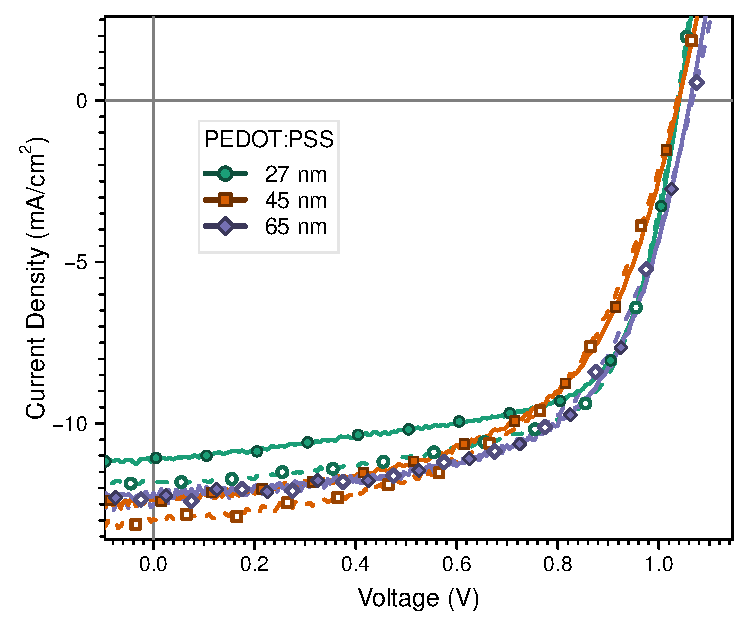
\includegraphics[width=0.8\textwidth]{jv_champions-pedotpss/pedotpss-IVs.pdf}
		\mycaption[Current-voltage sweeps for champion devices with different \glsentrytext{pedotpss} thicknesses.]{The solid line with filled markers represents the forward scan, while the dashed line with hollow markers represents the reverse scan.}\label{fig:thicknesses-jv_champions-pedotpss}
	\end{SCfigure}

	Using different spin coating speeds, devices with various \gls{pedotpss} thicknesses were obtained, as detailed in \cref{table:pedotpss_thickness}.
	The \gls{ito} roughness is small enough to make us certain that even the thinner, \SI{27}{\nm}, \gls{pedotpss} layer results in an homogeneous coverage.

	\paragraph{Current-voltage sweeps}
	In \cref{fig:thicknesses-jv_champions-pedotpss} we can observe the current-voltage sweeps of the champion devices while in \cref{table:thicknesses_jv} the averages and standard deviations are reported.
	None of the current\hyp{}voltage sweep parameters has shown a significant dependency on the \gls{pedotpss} \acr{htm} thickness.
	Indeed, the high holes mobility of \gls{pedotpss} \cite{Rutledge2013} was expected to make this layer to be a non\hyp{}limiting one.


	\begin{figure}
		\makebox[\textwidth][c]{
			\parbox{1.1\textwidth}{
				\centering
				\begin{subfigure}[t]{0.51\textwidth}
					\includegraphics[width=1.05\textwidth]{photophysics-pedotpss/photophysics-CEs.pdf}
					\subcaption{Charge from \acr{ce}}\label{fig:thicknesses-pedotpss-geometric-ce}
				\end{subfigure}
				\qquad
				\begin{subfigure}[t]{0.51\textwidth}
					\includegraphics[width=1.05\textwidth]{photophysics-pedotpss/photophysics-DCs-capacitance.pdf}
					\subcaption{Capacitance from \acr{dc}}\label{fig:thicknesses-pedotpss-geometric-dc}
				\end{subfigure}
				\mycaption[CE and DC of devices with different \glsentrytext{pedotpss} thicknesses, highlighting the varying geometric capacitance\index{geometric capacitance}.]{
					In (\textbf{a}) the charge \textsl{versus} light bias as obtained from \acr{ce} is reported. The upper solid lines are exponential fittings following \cref{eq:ce_full} while the bottom solid lines show just the exponential part, ignoring the geometric capacitance\index{geometric capacitance}. In (\textbf{b}) the capacitance dependence on light bias is reported as obtained from \acr{dc}. The solid line indicates the fitting using \cref{eq:dc_full}. All the fitted parameters are reported in \cref{table:thicknesses_photophysics}.
				}\label{fig:thicknesses-pedotpss-geometric}
			}
		}
	\end{figure}

	\paragraph{Geometric capacitance from \glsentryshort{dc} and \glsentryshort{ce}}
	Changing the \gls{pedotpss} \acr{htm} layer thickness did not affect the measured geometric capacitance\index{geometric capacitance} values reported in \cref{table:thicknesses_photophysics} and observable in \cref{fig:thicknesses-pedotpss-geometric}.
	This can either mean that no charge accumulates close to the \gls{ito}\-/\gls{pedotpss} interface (\textsl{e.g.}\ in case the two materials have the same workfunction) or, considering the series of parallel plate capacitors model, that this layer's large capacitance does not influence the total measured capacitance.

\section{Conclusions}
	We fabricated various top cathode perovskite solar cells varying the thickness of each solution deposited layer.
	We measured the geometric capacitance\index{geometric capacitance} of this set of devices using two independent characterisation techniques: \acr{ce} and \acr{dc}.
	From the obtained results, we gained insight on the storage location of the photogenerated charge at open circuit conditions.
	In our solar cell architecture, the holes are stored close to the \gls{pedotpss}\-/\gls{mapi} interface, likely in a thin depletion\index{space charge layer} layer in the \gls{htm}.
	Instead, the electrons does not get stored close to the \gls{mapi}\-/\gls{pcbm70} interface but either through the whole \acr{etm} layer or at the \gls{pcbm70}\-/\ch{Ag} interface.
	Likely, this is simply caused by a Debye length (space\index{space charge layer} charge layer width) larger than the \acr{etm} layer, due to the lack of doping in the \gls{pcbm70}.

